\section{Experiments}\label{sec:experiment}
% <<<<<<< HEAD
% We experimentally evaluated the performance and quality of our methodology \cref{subsec:heuristics},
% and compared it against the exhaustive approach in Section~\ref{TOADD}. In the following,
% \cref{subsec:experiments_infrastructure} presents the simulator and testing infrastructure adopted in our experiments, as well as the complete experimental settings; \cref{subsec:experiments_performance} analyses the performance of our solution in terms of execution time; \cref{subsec:experiments_quality} presents the quality of our heuristic algorithm in terms of the metrics in \cref{subsec:metrics}.

% \subsection{Testing Infrastructure and Experimental Settings}\label{subsec:experiments_infrastructure}
% Our testing infrastructure is a Swift-based simulator of a service-based ecosystem, including service execution, comparison, and composition. The simulator first defines the pipeline template as a sequence of vertexes in the range \hl{x-y}. We recall that alternative vertexes are modeled in different pipeline templates, while parallel vertexes only add a fixed execution time that is negligible and do not affect the quality of our approach. Each vertex is associated with a (set of) policy with transformations varying in three classes: \hl{a,b,c}. A set of functionally-equivalent candidate services is randomly generated, each service having a profile...\hl{to conclude}.
% Upon setting up the pipeline template, the sliding window size is configured and our methodology for pipeline instance generation starts. %The simulator selects a subset of vertexes along with their corresponding candidate services.
% The simulator calculates all possible pipeline instances, that is, it instantiates all vertexes with a service according to the selected window size. For each vertex, the simulator calculates a quality metric, selecting the first service from the optimal combination in the sliding window, then shifting the window by step 1.
% When the end of the vertex list is reached, or when the window size equals the vertex count, the simulator computes the optimal service combination for the remaining vertexes and the pipeline instance is generated.
% \hl{NON MI E' CHIARISSIMA To ensure that each service is interdependent within a combination, a hash function is employed. This function generates weights that services use to simulate transformations (data removal) mandated by the specified policies.}
% =======

We experimentally evaluated the performance and quality of our methodology, and corresponding heuristic implementation in \cref{subsec:heuristics},
and compare them against the exhaustive approach in Section~\ref{TOADD}. In the following,
\cref{subsec:experiments_infrastructure} presents the simulator and testing infrastructure adopted in our experiments, as well as the complete experimental settings; \cref{subsec:experiments_performance} analyses the performance of our solution in terms of execution time; \cref{subsec:experiments_quality} presents the quality of our heuristic algorithm in terms of the metrics in \cref{subsec:metrics}.

\subsection{Testing Infrastructure and Experimental Settings}\label{subsec:experiments_infrastructure}
Our testing infrastructure is a Swift-based simulator of a service-based ecosystem, including service execution, comparison, and composition.
The simulator first defines the pipeline template as a sequence of vertexes in the range $3-7$.
We recall that alternative vertexes are modeled in different pipeline templates,
while parallel vertexes only add a fixed execution time that is negligible and do not affect the quality of our approach.
Each vertex is associated with a (set of) policy with transformations varying in three classes:

\begin{itemize*}[label=roman*]
  \item \textit{Confident}: Adjusts data removal to a percentage within $[0.8,1]$.
  \item \textit{Diffident}: Sets data removal percentage to $[0.33,0.5]$.
  \item \textit{Average}: Modifies data removal percentage within $[0.33,1]$.
\end{itemize*}
set of functionally-equivalent candidate services is randomly generated.

Upon setting the sliding window size, the simulator selects a subset of vertexes along with their corresponding candidate services.
It then generates all possible service combinations for the chosen vertexes.
For each combination, the simulator calculates a metric, selecting the first service from the optimal combination before shifting the sliding window.
When the end of the vertex list is reached, or when the window size equals the vertex count, the simulator computes the optimal service combination for the remaining vertexes.

An hash function is to simulate the natural interdependence between services.
This is particularly important when the removal of data by one service may impact another.
By assigning weights to the services using this function, the system aims to reflect the interconnected dynamics among the services.

The simulator is used to assess the performance and quality of our sliding window heuristic in Section \ref{sec:heuristics} for the generation of the best pipeline instance (Section \ref{sec:instance}).
% Performance measures the heuristics execution time in different settings, while quality compares the results provided by our heuristics in terms of selected services with the optimal solution retrieved using the exhaustive approach.
%We note that the exhaustive approach generates the best pipeline instance by executing all possible combinations of candidate services.
%The emulator simplifies the execution of the service composition by removing the service selection phase, which is not relevant for the purpose of the experiment.
Our experiments have been run on a workstation equipped with a 2.40GHz i5-8279U CPU with 16GB RAM and a 512GB SSD.
Each experiment was repeated ten times and the results averaged to improve the reliability of the data.

\usetikzlibrary{positioning}
\usetikzlibrary{backgrounds}

\begin{figure}[!t]
  \centering

  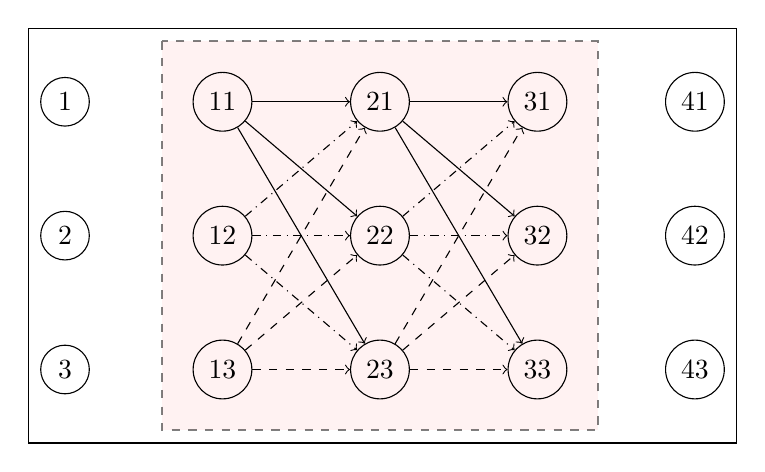
\begin{tikzpicture}[framed]
    \node[draw, circle] (s41) at (1,1.7) {$\sii{1}$};
    \node[draw, circle] (s42) at (1,0) {$\sii{2}$};
    \node[draw, circle] (s43) at (1,-1.7) {$\sii{3}$};

    \node[draw, circle] (s1) at (3,1.7) {$\sii{11}$};
    \node[draw, circle] (s2) at (3,0) {$\sii{12}$};
    \node[draw, circle] (s3) at (3,-1.7) {$\sii{13}$};

    \node[draw, circle] (s11) at (5,1.7) {$\sii{21}$};
    \node[draw, circle] (s12) at (5,0) {$\sii{22}$};
    \node[draw, circle] (s13) at (5,-1.7) {$\sii{23}$};

    \node[draw, circle] (s21) at (7,1.7) {$\sii{31}$};
    \node[draw, circle] (s22) at (7,0) {$\sii{32}$};
    \node[draw, circle] (s23) at (7,-1.7) {$\sii{33}$};

    \node[draw, circle] (s31) at (9,1.7) {$\sii{41}$};
    \node[draw, circle] (s32) at (9,0) {$\sii{42}$};
    \node[draw, circle] (s33) at (9,-1.7) {$\sii{43}$};


    % \draw[->] (node2) -- (node3);
    \draw[->] (s1) -- (s11);
    \draw[->] (s1) -- (s12);
    \draw[->] (s1) -- (s13);

    \draw[->,dashdotted] (s2) -- (s11);
    \draw[->,dashdotted] (s2) -- (s12);
    \draw[->,dashdotted] (s2) -- (s13);

    \draw[->,dashed] (s3) -- (s11);
    \draw[->,dashed] (s3) -- (s12);
    \draw[->,dashed] (s3) -- (s13);


    \draw[->] (s11) -- (s21);
    \draw[->] (s11) -- (s22);
    \draw[->] (s11) -- (s23);

    \draw[->,dashdotted] (s12) -- (s21);
    \draw[->,dashdotted] (s12) -- (s22);
    \draw[->,dashdotted] (s12) -- (s23);

    \draw[->,dashed] (s13) -- (s21);
    \draw[->,dashed] (s13) -- (s22);
    \draw[->,dashed] (s13) -- (s23);


    \begin{scope}[on background layer]
      \draw[thick, dashed, fill=red!10, opacity=0.5]
      ([shift={(-0.5,0.5)}]s1.north west) rectangle ([shift={(0.5,-0.5)}]s23.south east);

    \end{scope}
  \end{tikzpicture}
  \caption{Service composition instance}
  \label{fig:service_composition_instance}
\end{figure}

\subsection{Perfomance}\label{subsec:experiments_performance}
% \subsection{performance}
% \begin{itemize}
%   \item Finestra scorrevole da 1 a N=Nodi
%   \item Servizi 5 a 20 passo 5 + 50??
%   \item
% \end{itemize}
% \subsection{Metriche/Euristiche}
We first calculated the execution time required by our exhaustive solution.
We incrementally varied the number of vertexes and the number of services per vertex.
The results of these evaluations are presented in \cref{fig:perf_exhaustive}.
As anticipated, the trend in execution times is exponential. \cref{fig:perf_exhaustive} displays the execution time plots,
clearly showing that as the number of vertexes increases, the execution time grows exponentially.
Execution times for up to 5 vertexes and 6 services were computed directly,
while the remaining data points were obtained through interpolation.
Subsequently, the logical extension of this empirical inquiry involves evaluating the execution time efficiency attributable to the implementation of the sliding window heuristic.

We then evaluated our heuristics to quantify the execution time reduction achieved through the application of heuristics.
In this context, the number of vertexes and services per vertex was incrementally increased,
with the addition of a sliding window whose size was progressively enlarged in each experiment.
The outcomes are depicted in \cref{fig:perf_window}, and as expected,
we observed a marked reduction in execution times with the implementation of the sliding window heuristic.
This empirical evidence highlights the heuristic's ability to reduce computational demands,
an aspect that becomes increasingly pivotal as the problem's complexity grows.
The use of a logarithmic scale to illustrate the results linearizes the exponential growth associated with the exhaustive method,
offering a clear visual confirmation of the heuristic's efficiency in decreasing computational time.


\subsection{Quality}\label{subsec:experiments_quality}
We finally evaluated the quality of our heuristic comparing, where possible, its results with the optimal solution retrieved by executing the exhaustive approach. The latter executes with window size equals to the number of vertexes in the pipeline template, and provides the best, among all possible, solutions.

We run our experiments in the three settings in Section \ref{}, namely, confident, diffident, average, and varied: \emph{i)} the number of vertexes in the pipeline template in [3,6], \emph{ii)} the window size in [1,$|$max$_v$$|$], where max$_v$ is the number of vertexes in the pipeline template, and \emph{iii)} the number of candidate services for each vertex in the pipeline template in [2, 6].

\cref{fig:quality_window_bad,fig:quality_window_average,fig:quality_window_good} presents our results using metric Jensen-Shannon Divergence.
%
When a diffident setting is used, \cref{fig:quality_window_bad}, the quality range from 0.7 to 0.9, with the highest quality retrieved for the pipeline template with 3 vertices and the lowest with 7 vertices.
In particular, the quality ranges from 0.88 (greedy approach) to 0.93 (exhaustive approach) for a 3-vertex pipeline with a loss of 5,38\% in the worst case, from 0.84 to 0.92 for a 4-vertex pipeline with a loss of 8,7\%, from 0.84 to 0.89 for a 5-vertex pipeline with a loss of 5,61\%, from 0.8 to 0.89 for a 6-vertex pipeline with a loss of 10,11\%, and from 0.72 to 0.88 for a 7-vertex pipeline with a loss of 18,18\%. We note that the benefit of an increasing window size can be appreciated with lower numbers, reaching a sort of saturation around the average length (e.g., window of length 4 with a 7-vertex pipeline) where the quality with different length almost overlaps. The only exception is for 6-vertex pipeline where the overapping starts with window size 2. However, this might be due to the specific setting and therefore does not generalize.
%Thus because the heuristic has more services to choose from and can find a better combination.
We also observe that, as the window size increase, the quality increase as well. This suggests that the heuristic performs better when it has a broader perspective of the data it is governing.

\hl{QUESTO E' PIU' DA CONCLUSIONE FINALE.} Finally, the data suggest that while larger window sizes generally lead to better performance, there might exist a point where the balance between window size and performance is optimized. Beyond this point, the incremental gains in metric values may not justify the additional computational resources or the complexity introduced by larger windows.


\begin{figure*}[ht]
  \centering
  \begin{subfigure}{0.33\textwidth}
    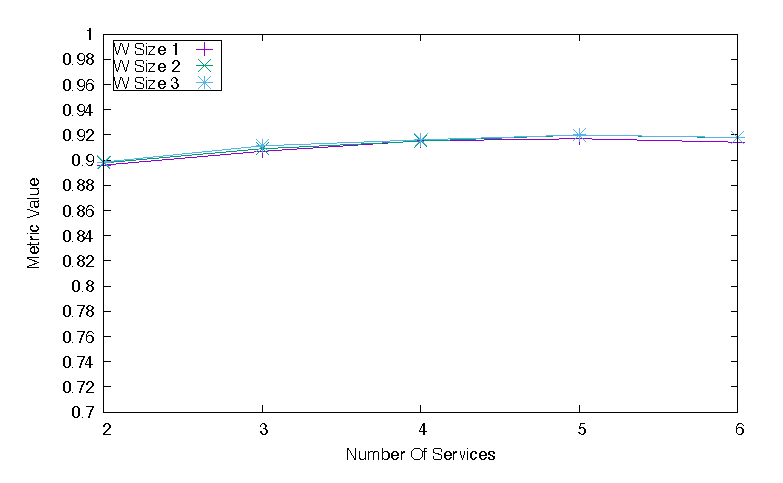
\includegraphics[width=\textwidth]{Images/graphs/quality_plot_average_n3.eps}
    \caption{3 vertices}
    \label{fig:first}
  \end{subfigure}
  \hfill
  \begin{subfigure}{0.33\textwidth}
    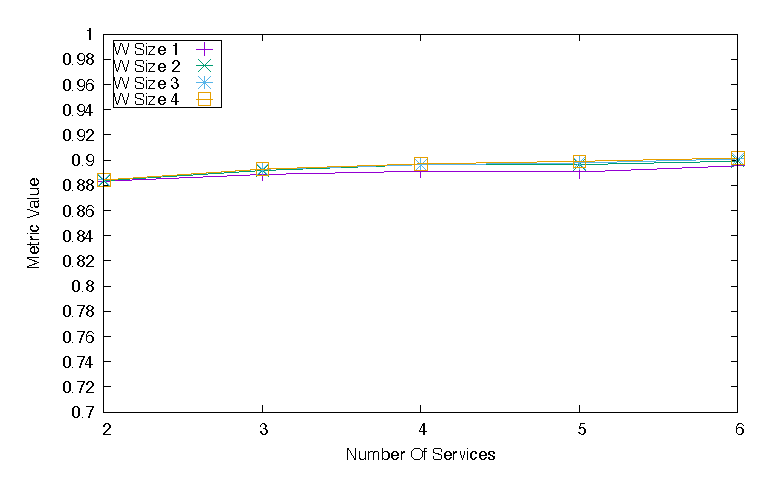
\includegraphics[width=\textwidth]{Images/graphs/quality_plot_average_n4.eps}
    \caption{4 vertices}
    \label{fig:second}
  \end{subfigure}
  \hfill
  \begin{subfigure}{0.33\textwidth}
    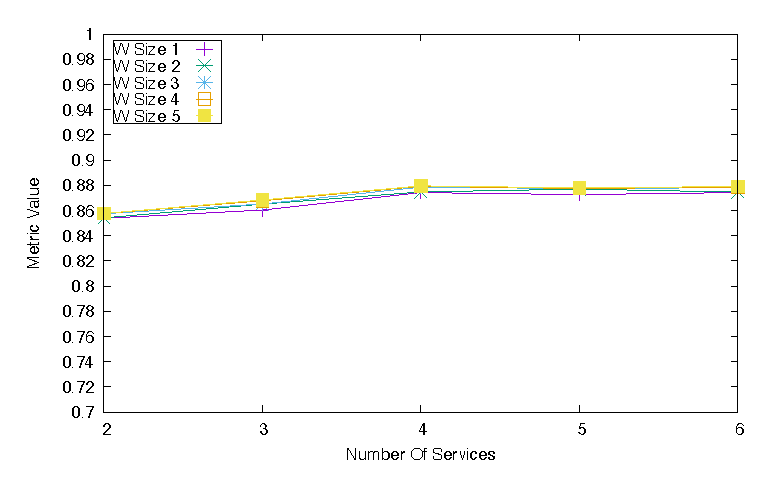
\includegraphics[width=\textwidth]{Images/graphs/quality_plot_average_n5.eps}
    \caption{5 vertices}
    \label{fig:third}
  \end{subfigure}
  \hfill
  \begin{subfigure}{0.33\textwidth}
    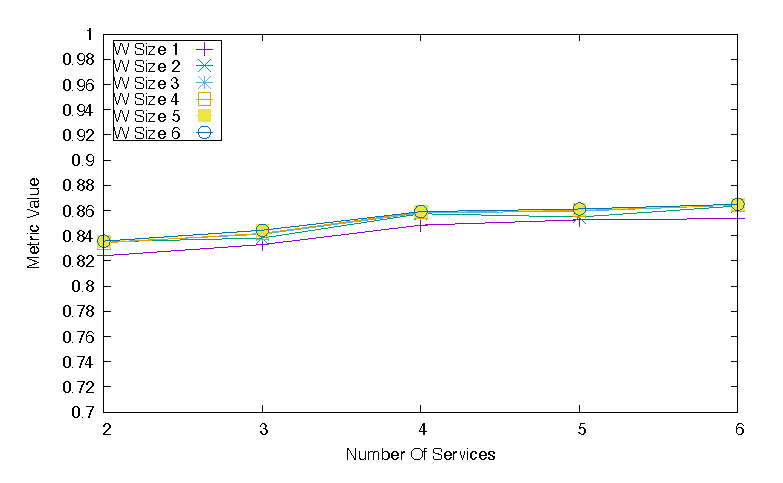
\includegraphics[width=\textwidth]{Images/graphs/quality_plot_average_n6.eps}
    \caption{6 vertices}
    \label{fig:third}
  \end{subfigure}
  % \hfill
  % \begin{subfigure}{0.33\textwidth}
  %   \includegraphics[width=\textwidth]{Images/graphs/quality_plot_average_n7.eps}
  %   \caption{7 vertices}
  %   \label{fig:third}
  % \end{subfigure}
  \caption{ Quality evaluation with \textit{Confident} profile.}
  \label{fig:quality_window_good}
\end{figure*}

\begin{figure*}[ht]
  \centering
  \begin{subfigure}{0.33\textwidth}
    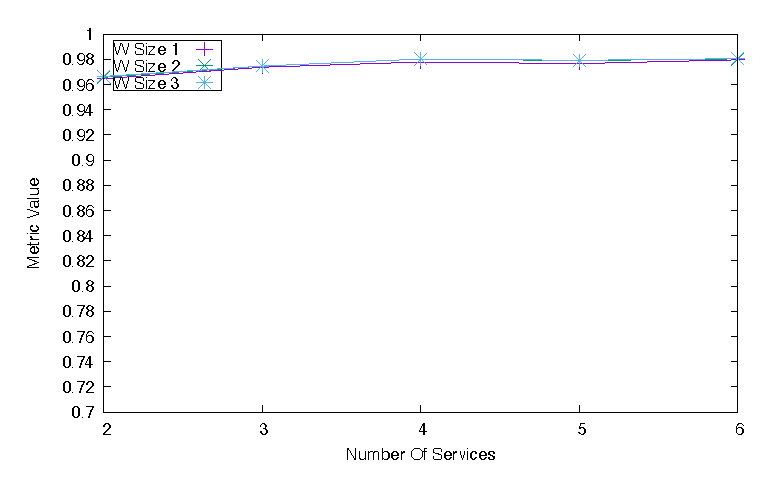
\includegraphics[width=\textwidth]{Images/graphs/quality_plot_good_n3.eps}
    \caption{3 vertices}
    \label{fig:first}
  \end{subfigure}
  \hfill
  \begin{subfigure}{0.33\textwidth}
    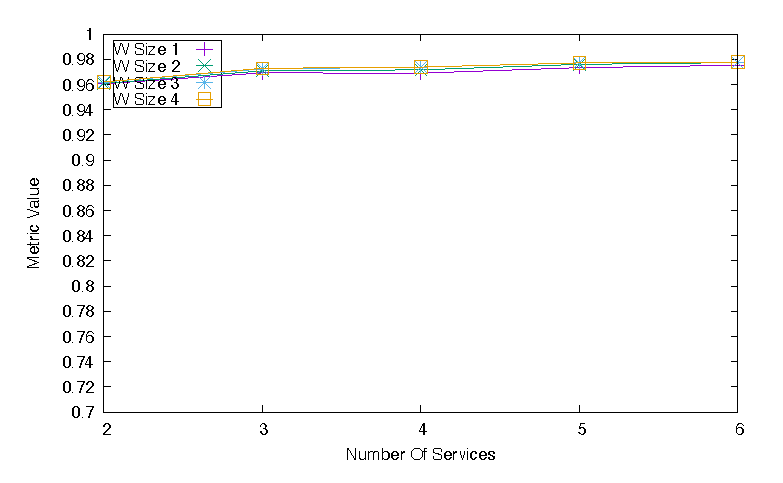
\includegraphics[width=\textwidth]{Images/graphs/quality_plot_good_n4.eps}
    \caption{4 vertices}
    \label{fig:second}
  \end{subfigure}
  \hfill
  \begin{subfigure}{0.33\textwidth}
    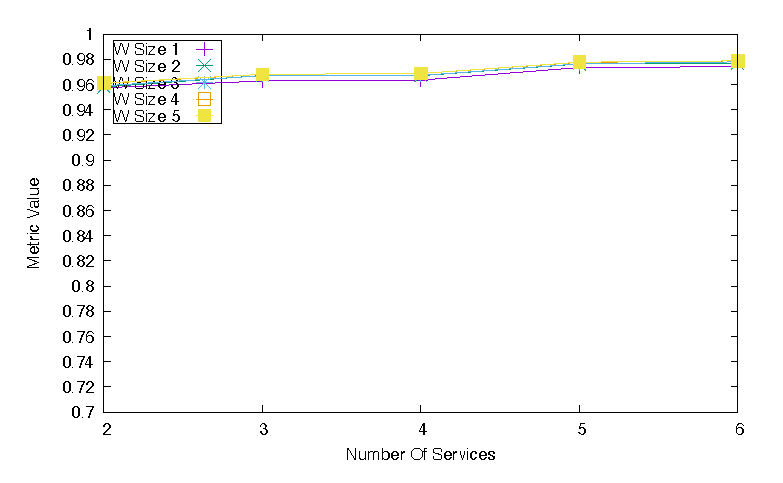
\includegraphics[width=\textwidth]{Images/graphs/quality_plot_good_n5.eps}
    \caption{5 vertices}
    \label{fig:third}
  \end{subfigure}
  \hfill
  \begin{subfigure}{0.33\textwidth}
    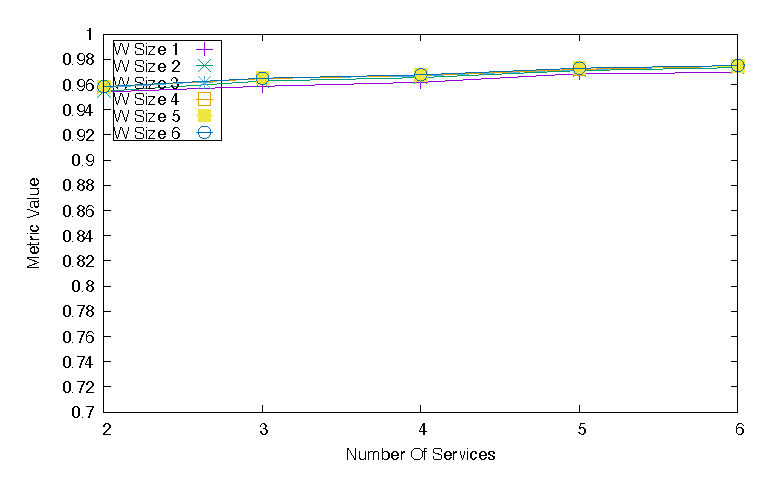
\includegraphics[width=\textwidth]{Images/graphs/quality_plot_good_n6.eps}
    \caption{6 vertices}
    \label{fig:third}
  \end{subfigure}
  \hfill
  \begin{subfigure}{0.33\textwidth}
    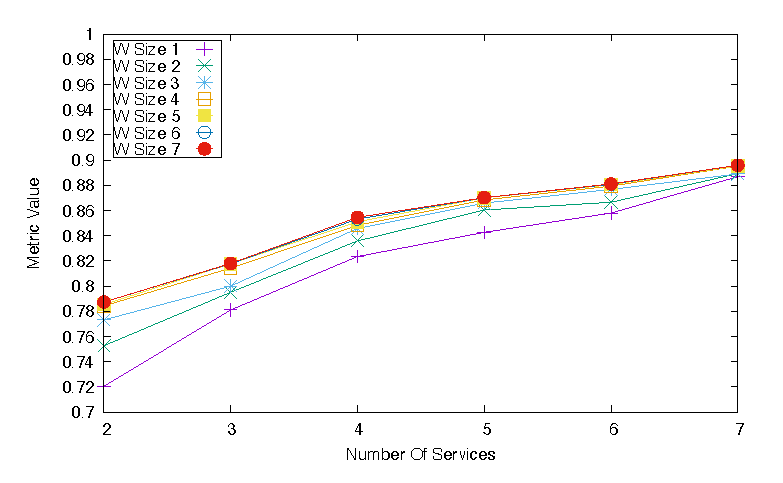
\includegraphics[width=\textwidth]{Images/graphs/quality_plot_vbad_n7.eps}
    \caption{7 vertices}
    \label{fig:third}
  \end{subfigure}
  \caption{Quality evaluation with \textit{Average} profile.}
  \label{fig:quality_window_average}
\end{figure*}


\begin{figure*}[ht!]
  \centering
  \begin{subfigure}{0.33\textwidth}
    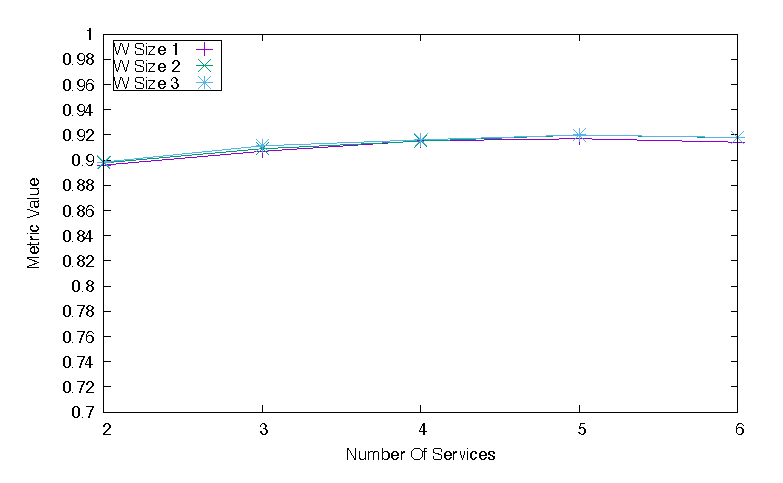
\includegraphics[width=\textwidth]{Images/graphs/quality_plot_bad_n3.eps}
    \caption{3 vertices}
    \label{fig:quality_window_bad_a}
  \end{subfigure}
  \hfill
  \begin{subfigure}{0.33\textwidth}
    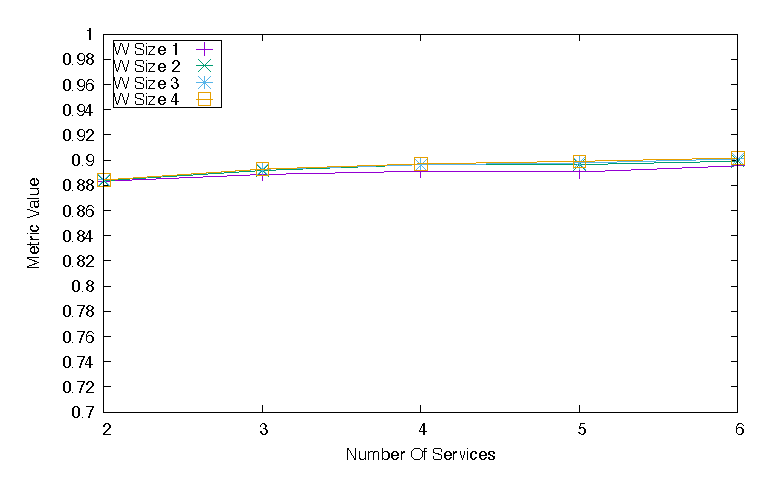
\includegraphics[width=\textwidth]{Images/graphs/quality_plot_bad_n4.eps}
    \caption{4 vertices}
    \label{fig:quality_window_bad_b}
  \end{subfigure}
  \hfill
  \begin{subfigure}{0.33\textwidth}
    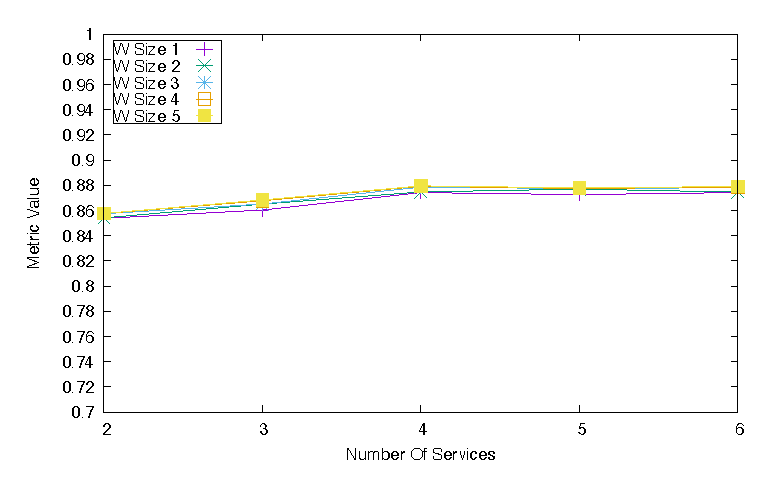
\includegraphics[width=\textwidth]{Images/graphs/quality_plot_bad_n5.eps}
    \caption{5 vertices}
    \label{fig:quality_window_bad_c}
  \end{subfigure}
  \hfill
  \begin{subfigure}{0.33\textwidth}
    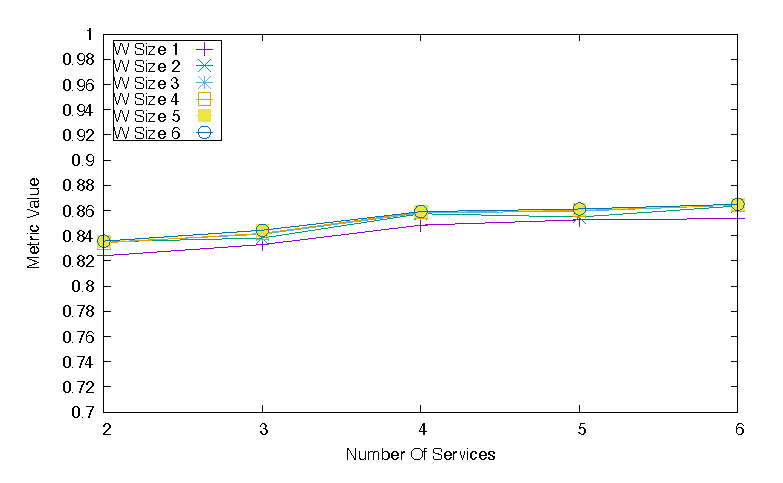
\includegraphics[width=\textwidth]{Images/graphs/quality_plot_bad_n6.eps}
    \caption{6 vertices}
    \label{fig:quality_window_bad_d}
  \end{subfigure}
  % \hfill
  % \begin{subfigure}{0.33\textwidth}
  %   \includegraphics[width=\textwidth]{Images/graphs/quality_plot_bad_n7.eps}
  %   \caption{7 vertices}
  %   \label{fig:quality_window_bad_e}
  % \end{subfigure}

  \caption{Quality evaluation with \textit{Diffident} profile.}
  \label{fig:quality_window_bad}
\end{figure*}


\begin{figure*}[ht!]
  \centering
  \begin{subfigure}{0.33\textwidth}
    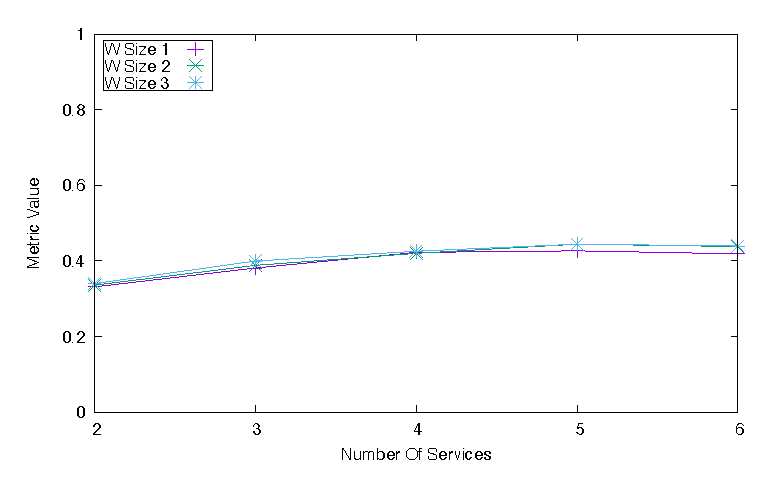
\includegraphics[width=\textwidth]{Images/graphs/quality_plot_bad_percentage_n3.eps}
    \caption{3 vertices}
    \label{fig:quality_window_bad_percentage_a}
  \end{subfigure}
  \hfill
  \begin{subfigure}{0.33\textwidth}
    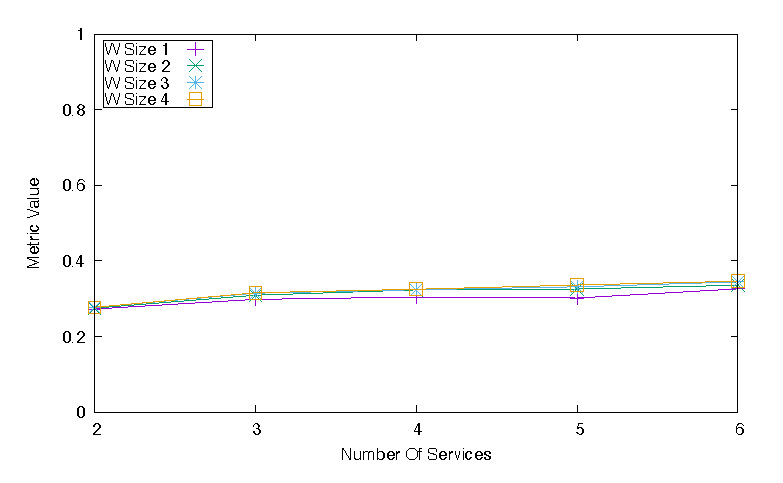
\includegraphics[width=\textwidth]{Images/graphs/quality_plot_bad_percentage_n4.eps}
    \caption{4 vertices}
    \label{fig:quality_window_bad_percentage_b}
  \end{subfigure}
  \hfill
  \begin{subfigure}{0.33\textwidth}
    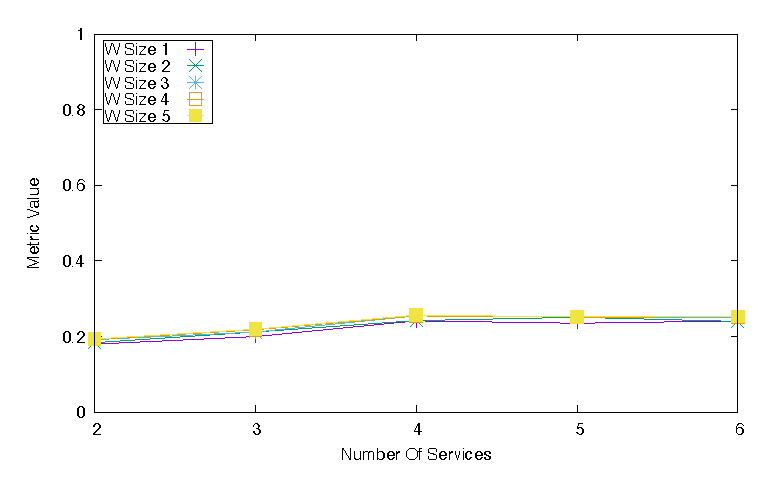
\includegraphics[width=\textwidth]{Images/graphs/quality_plot_bad_percentage_n5.eps}
    \caption{5 vertices}
    \label{fig:quality_window_bad_percentage_c}
  \end{subfigure}
  \hfill
  \begin{subfigure}{0.33\textwidth}
    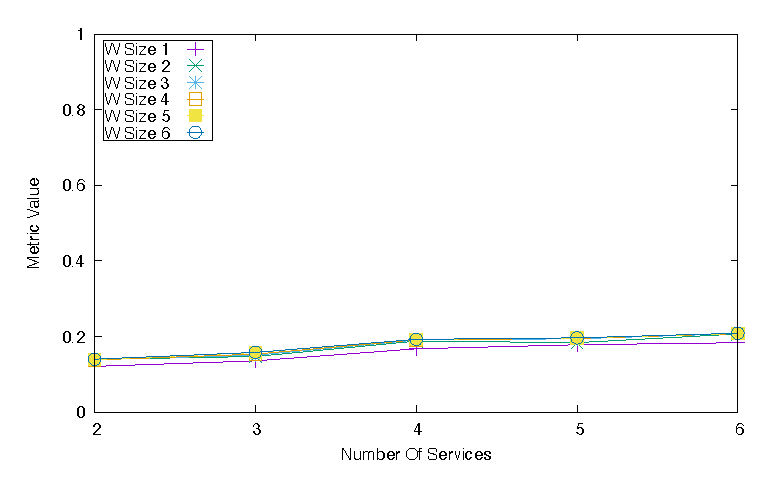
\includegraphics[width=\textwidth]{Images/graphs/quality_plot_bad_percentage_n6.eps}
    \caption{6 vertices}
    \label{fig:quality_window_bad_percentage_d}
  \end{subfigure}
  % \hspace{0.04\textwidth}
  % \begin{subfigure}{0.33\textwidth}
  %   \includegraphics[width=\textwidth]{Images/graphs/quality_plot_bad_n7.eps}
  %   \caption{7 vertices}
  %   \label{fig:quality_window_bad_percentage_e}
  % \end{subfigure}

  \caption{Quality Percentage evaluation with \textit{Diffident} profile.}
  \label{fig:quality_window_bad_percentage}
\end{figure*}

% % We recall that we considered three different setting, confident, diffident, average, varying the policy transformations, that is, the amount of data removal at each vertex. Setting confident assigns to each policy a transformation that changes the amount of data removal in the interval [x,y] (Jaccard coefficient) or decreases the probability distribution dissimilarity in the interval [x,y] (Jensen-Shannon Divergence). Setting diffident assigns to each policy a transformation that changes the amount of data removal in the interval [x,y] (Jaccard coefficient) or decreases the probability distribution dissimilarity in  the interval [x,y] (Jensen-Shannon Divergence). Setting average assigns to each policy a transformation that changes the amount of data removal in the interval [x,y] (Jaccard coefficient) or decreases the probability distribution dissimilarity in  the interval [x,y] (Jensen-Shannon Divergence).
% We finally evaluated the quality of our heuristic comparing, where possible,
% its results with the optimal solution retrieved by executing the exhaustive approach.
% The latter executes with window size equals to the number of services per vertex and provides the best,
% among all possible, solution.

% The number of vertexes has been varied from 3 to 7, while the number of services per vertex has been set from 2 to 6.
% The experiments have been conducted with different service data pruning profiles.

% \hl{DOBBIAMO SPIEGARE COSA ABBIAMO VARIATO NEGLI ESPERIMENTI E COME, WINDOW SIZE, NODI, ETC.

%   LE IMMAGINI CHE ABBIAMO SONO SOLO QUELLE 5? POSSIAMO ANCHE INVERTIRE GLI ASSI E AGGIUNGERE VISUALI DIVERSE}

% <<<<<<< HEAD
% \cref{fig:quality_window} presents our results with setting \hl{confident} and metric Jaccard coefficient. \cref{fig:quality_window}(a)--(e) \hl{aggiungere le lettere e uniformare l'asse y} present the retrieved quality varying the number of vertexes in [3, 7], respectively. Each figure in \cref{fig:quality_window}(a)--(e) varies the number of candidate services at each node in the range [2, 6] and the window size W in the range [1, $|$vertexes$|$].
% \hl{aggiungiamo i numeri piu significativi (asse y).}
% From the results, some clear trends emerge. As the number of vertexes increases, the metric values tend to decrease (better data quality) as the window size increases across different node configurations.
% This suggests that the heuristic performs better when it has a broader perspective of the data and services. The trend is consistent across all node cardinalities (from three to seven), indicating that the heuristic's enhanced performance with larger window sizes is not confined to a specific setup but rather a general characteristic of its behavior.
% Finally, the data suggest that while larger window sizes generally lead to better performance,
% there might exist a point where the balance between window size and performance is optimized. \hl{For instance, ...}
% Beyond this point, the incremental gains in metric values may not justify the additional computational resources or the complexity introduced by larger windows.

% \hl{RIPETERE PER TUTTI I SETTINGS}


% \begin{figure}
%   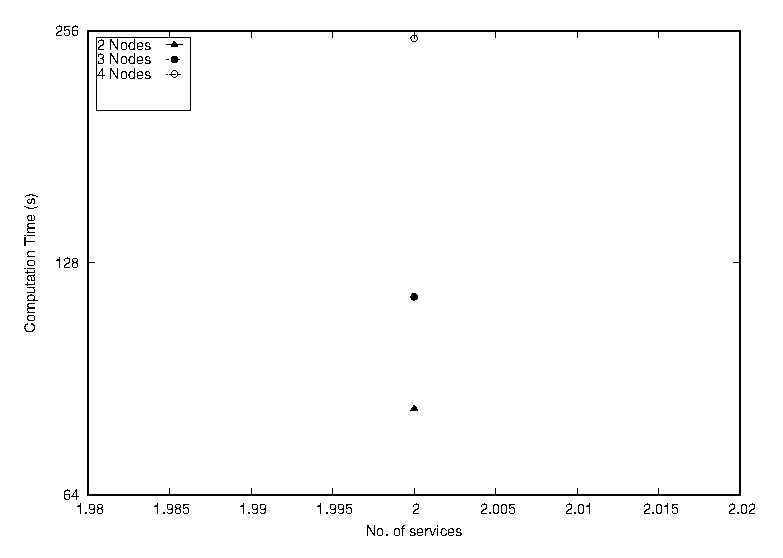
\includegraphics[width=0.95\columnwidth]{graphs/exhaustive_performance.eps}
%   \caption{Exhaustive execution time evaluation. The x-axis represents the number of services, while the y-axis represents the execution time in seconds. The execution time is expressed both in linear and logarithmic scales.}
%   \label{fig:perf_exhaustive}
% \end{figure}

% \begin{figure}[!t]
%   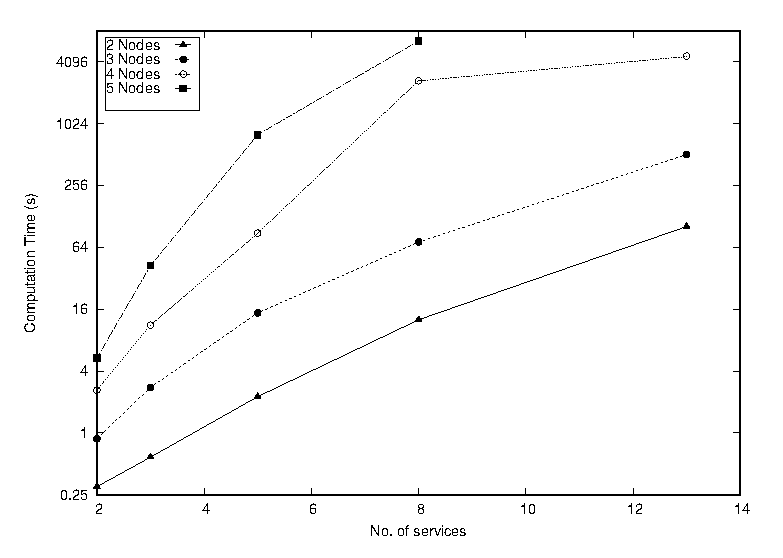
\includegraphics[width=0.95\columnwidth]{graphs/window_performance.eps}
%   \caption{Preliminary performance evaluation.\hl{METTERE LE 4 IMG NON UN'UNICA EPS}}
%   \label{fig:perf_window}
% \end{figure}


% \begin{figure}[!t]
%   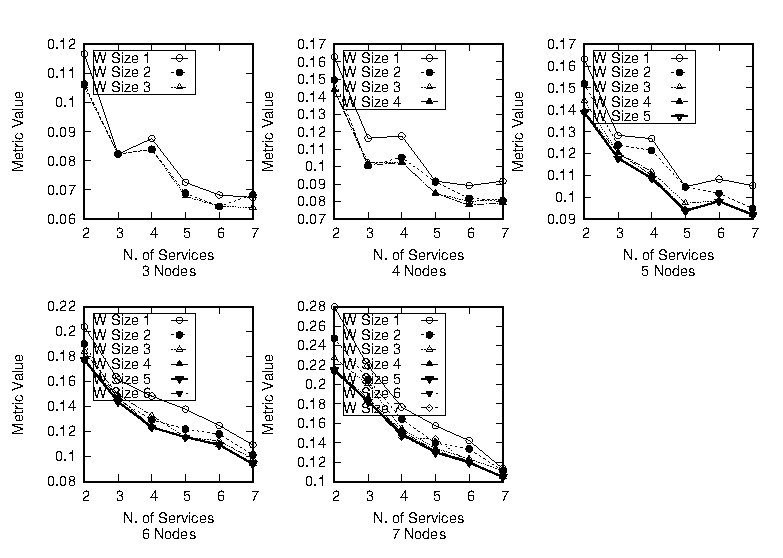
\includegraphics[width=0.95\columnwidth]{graphs/window_quality.eps}
%   \caption{Quality evaluation.\hl{METTERE LE 4 IMG NON UN'UNICA EPS}}
%   \label{fig:quality_window}
% \end{figure}
%=======


%In the figures each chart represents a configuration with a specific number of vertexes, ranging from 3 to 7. On the x-axis, the number of services is plotted, which ranges from 2 to 7. The y-axis represents the metric value. Each chart shows different window sizes, labeled as W Size 1, W Size 2, and so on, up to the maximum window size.
